\documentclass[a4paper,12pt]{article}
\usepackage[utf8]{inputenc}
\usepackage[LGR,T1]{fontenc}
\usepackage{alphabeta}
\usepackage{amsmath}
\usepackage{float}
\usepackage{multirow}
\usepackage{amsfonts}
\usepackage{amssymb}
\usepackage{graphicx}
\usepackage{listings}
\usepackage{booktabs}  % For better looking tables
\usepackage{hyperref}
\usepackage{xcolor}

\lstset{
  basicstyle=\ttfamily\footnotesize,
  keywordstyle=\color{blue},
  commentstyle=\color{gray},
  stringstyle=\color{red},
  showstringspaces=false,
  breaklines=true,
  frame=single,
  language=R,
  extendedchars=true,
  literate={β}{{\beta}}1
}

\title{Αναγνώριση Προτύπων \\ 1η Εργαστηριακή Άσκηση \\ Χειμερινό Εξάμηνο 2024-2025 \\ Ε.ΔE.ΜΜ}
\author{Σπανάκης Παναγιώτης-Αλέξιος (ΑΜ: 03400274) \\ }
\date{08/11/2024}

\begin{document}

\maketitle
\section*{Βήμα 1}

\begin{table}[h!]
    \centering
    \begin{tabular}{|c|c|c|c|c|c|}
        \hline
        \textbf{Vowel}      & \textbf{Speaker} & \textbf{Pitch (Hz)} & \textbf{F1 (Hz)} & \textbf{F2 (Hz)} & \textbf{F3 (Hz)} \\ \hline
        \multirow{2}{*}{α}  & man              & 134.06              & 777.91           & 1217.69          & 2405.49          \\ \cline{2-6}
                            & woman            & 176.84              & 859.08           & 1837.31          & 3146.39          \\ \hline
        \multirow{2}{*}{ου} & man              & 130.65              & 372.17           & 1788.73          & 2327.56          \\ \cline{2-6}
                            & woman            & 184.51              & 321.15           & 1566.12          & 2631.54          \\ \hline
        \multirow{2}{*}{ι}  & man              & 132.04              & 387.10           & 2047.69          & 2556.83          \\ \cline{2-6}
                            & woman            & 178.49              & 368.76           & 2259.41          & 2951.24          \\ \hline
    \end{tabular}
    \caption{Measurements for vowels by male and female speakers.}
    \label{tab:vowels}
\end{table}

\textbf{Αρχικά, Σύγκριση Θεμελιώδους Συχνότητας (Pitch):}
Όπως αναμενόταν, η μέση συχνότητα της γυναικείας ομιλήτριας (Ομιλητής 2) είναι αισθητά υψηλότερη από εκείνη του ανδρικού ομιλητή (Ομιλητής 1)
για όλα τα φωνήεντα. Συγκεκριμένα, για το φωνήεν \textbf{"α"} ο άντρας έχει 134 Hz ενώ η γυναίκα 177 Hz, για το \textbf{"ου"} ο
άντρας έχει 131 Hz ενώ η γυναίκα 185 Hz, και για το \textbf{"ι"} ο άντρας 132 Hz έναντι της γυναίκας στα 178 Hz.
Αυτή η διαφορά είναι σύμφωνη με τις γενικές φωνητικές τάσεις όπου οι γυναίκες έχουν υψηλότερες συχνότητες λόγω ανατομικών διαφορών,
όπως οι μικρότερες και πιο τεντωμένες φωνητικές χορδές.

\textbf{Παρατηρήσεις για τα Formants:}
Οι τιμές των μορφάντων (F1, F2, F3) είναι επίσης υψηλότερες για τη γυναίκα ομιλήτρια συγκριτικά με τον άντρα,
κάτι που αναμένεται λόγω του μικρότερου φωνητικού σωλήνα, ο οποίος επηρεάζει τις συχνότητες αντήχησης και οδηγεί σε
μεγαλύτερες τιμές για τα formants. Για παράδειγμα, για το φωνήεν \textbf{"α"}, η πρώτη μορφάντις (F1) του άνδρα είναι
778 Hz, ενώ της γυναίκας είναι 859 Hz. Παρόμοια, η δεύτερη μορφάντις (F2) του άνδρα είναι 1218 Hz ενώ της γυναίκας
1837 Hz, και η τρίτη (F3) του άνδρα είναι 2405 Hz έναντι 3146 Hz για τη γυναίκα. Το ίδιο μοτίβο παρατηρείται και στα υπόλοιπα φωνήεντα.

\textbf{Ειδικές Παρατηρήσεις ανά Φωνήεν:}
\begin{itemize}
    \item Για το \textbf{"α"}, παρατηρούμε υψηλότερη F1 και F2 και στους δύο ομιλητές σε σχέση με τα φωνήεντα "ου" και "ι", κάτι που δείχνει ότι το "α" είναι πιο ανοιχτό και κεντρικό φωνήεν. Οι σημαντικά υψηλότερες τιμές F2 και F3 για τη γυναίκα ομιλήτρια πιθανώς υποδεικνύουν μια πιο πρόσθια εκφορά.
    \item Το \textbf{"ου"} εμφανίζει τη χαμηλότερη F1 και στους δύο ομιλητές, κάτι που δείχνει πως πρόκειται για ένα πιο κλειστό και οπίσθιο φωνήεν. Η διαφορά της F2 ανάμεσα στους ομιλητές ενισχύει την οπίσθια θέση του φωνήεντος και για τα δύο φύλα.
    \item Για το \textbf{"ι"}, παρατηρείται υψηλή F2, ειδικά για τη γυναίκα, κάτι που συνάδει με τον πρόσθιο, υψηλό χαρακτήρα του φωνήεντος αυτού. Η κοντινή απόσταση μεταξύ F2 και F3 στη γυναικεία φωνή μπορεί να υποδηλώνει μια πιο έντονη εκφορά.
\end{itemize}

\textbf{Γενικές Διαφορές μεταξύ των Φύλων:}
Οι διαφορές στις συχνότητες της θεμελιώδους συχνότητας και των μορφάντων που παρατηρήθηκαν είναι σύμφωνες με τις κοινές φωνητικές διακρίσεις μεταξύ ανδρικών και γυναικείων φωνών, με τον ανδρικό ομιλητή να εμφανίζει χαμηλότερες συχνότητες σε όλες τις παραμέτρους.

\section*{Βήμα 2}

Η συνάρτηση \texttt{data\_parser(directory)} λειτουργεί ως εξής:

\begin{enumerate}
    \item \textbf{Αρχικοποίηση}: Δημιουργεί τρεις κενές λίστες (\texttt{wavs}, \texttt{speakers}, \texttt{digits}).
    \item \textbf{Διάβασμα Αρχείων}: Διατρέχει όλα τα αρχεία στον καθορισμένο κατάλογο.
    \item \textbf{Φόρτωση Ήχου}: Φορτώνει κάθε αρχείο ήχου με συχνότητα 16kHz και προσθέτει τα δεδομένα στη λίστα \texttt{wavs}.
    \item \textbf{Εξαγωγή Πληροφοριών}: Από το όνομα του αρχείου, χρησιμοποιεί κανονική έκφραση για να εξάγει το ψηφίο και τον αριθμό του ομιλητή, τα οποία προστίθενται στις λίστες \texttt{digits} και \texttt{speakers} αντίστοιχα.
    \item \textbf{Επιστροφή Αποτελεσμάτων}: Επιστρέφει τις τρεις λίστες με τα ηχητικά δεδομένα, τους ομιλητές και τα ψηφία.
\end{enumerate}

\section*{Βήμα 3}

Η συνάρτηση \texttt{extract\_mfccs(wavs)} λειτουργεί ως εξής:

\begin{enumerate}
    \item \textbf{Αρχικοποίηση}: Δημιουργεί μια κενή λίστα \texttt{mfccs} για την αποθήκευση των χαρακτηριστικών.
    \item \textbf{Εξαγωγή MFCCs}: Για κάθε ήχο στη λίστα \texttt{wavs}, εξάγει 13 Mel-Frequency Cepstral Coefficients (MFCCs) χρησιμοποιώντας παράθυρο μήκους 25 ms και βήμα 10 ms (\texttt{n\_fft=400}, \texttt{hop\_length=160}).
    \item \textbf{Υπολογισμός Deltas}: Υπολογίζει την πρώτη (\texttt{delta}) και δεύτερη (\texttt{delta2}) τοπική παράγωγο των MFCCs.
    \item \textbf{Αποθήκευση Χαρακτηριστικών}: Προσθέτει τα MFCCs, τα deltas και τα delta-deltas ως ένα tuple στη λίστα \texttt{mfccs}.
    \item \textbf{Επιστροφή Αποτελεσμάτων}: Επιστρέφει τη λίστα \texttt{mfccs} με τα εξαγόμενα χαρακτηριστικά για κάθε αρχείο ήχου.
\end{enumerate}

\section*{Βήμα 4}

Τα ψηφία που αναλύθηκαν είναι $n1=7$ και $n2=4$ του 1ου και 2ου MFCC αντίστοιχα. Τα ιστογράμματα των ψηφίων αυτών για τα πρώτα 2 MFCCs παρουσιάζονται στα
Σχήματα \ref{fig:hist1} και \ref{fig:hist2}. Η διακύμανση των MFCCs για τα δύο ψηφία φαίνεται στον πίνακα \ref{tab:variance}.

\begin{figure}[H]
    \centering
    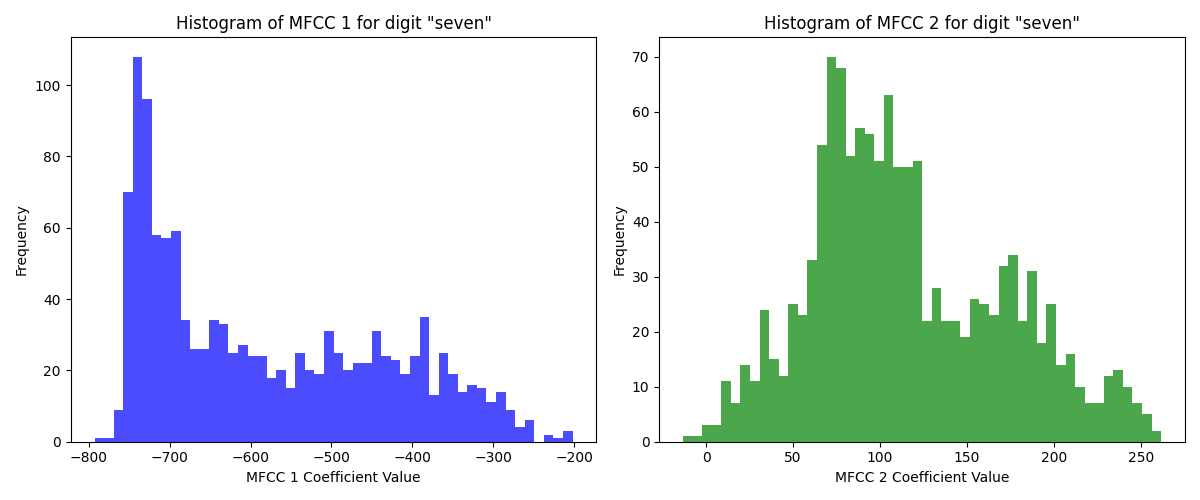
\includegraphics[width=\textwidth]{images/histograms_seven.png}
    \caption{Ιστόγραμμα του ψηφίου "seven" για τους δύο MFCCs.}
    \label{fig:hist1}
\end{figure}

\begin{figure}[H]
    \centering
    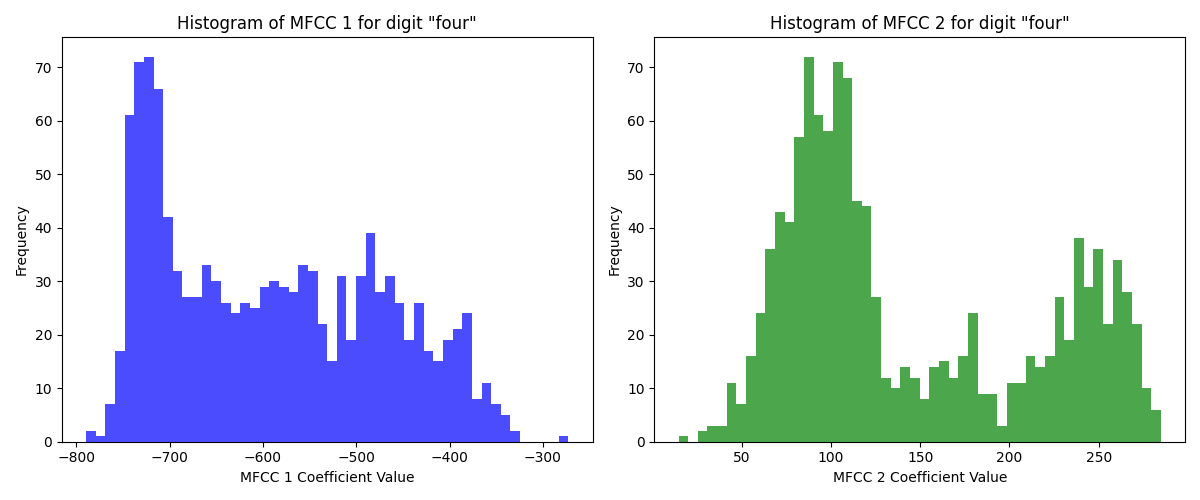
\includegraphics[width=\textwidth]{images/histograms_four.png}
    \caption{Ιστόγραμμα του ψηφίου "four" για τους δύο MFCCs.}
    \label{fig:hist2}
\end{figure}

\begin{table}
    \centering
    \begin{tabular}{|c|c|c|}
        \hline
        \textbf{Digit} & \textbf{MFCC 1} & \textbf{MFCC 2} \\ \hline
        seven          & 21497.80        & 3068.08         \\ \hline
        four           & 14009.79        & 4906.44         \\ \hline
    \end{tabular}
    \caption{Variance of MFCCs for digits "seven" and "four".}
    \label{tab:variance}
\end{table}

Mπορούμε να εξάγουμε τα εξής συμπεράσματα:

Πρώτον, παρατηρείται σημαντική διαφορά στη διακύμανση των δύο πρώτων MFCC χαρακτηριστικών μεταξύ των ψηφίων "seven" και "four".
Συγκεκριμένα, το MFCC1 του "seven" παρουσιάζει πολύ μεγαλύτερη διακύμανση σε σύγκριση με το "four" (21497.80 έναντι 14008.79),
ενώ η διακύμανση του MFCC2 παρουσιάζει επίσης διαφορά, αν και μικρότερη (3068.08 για το "seven" και 4096.44 για το "four").

Δεύτερον, τα ιστογράμματα των MFCC1 και MFCC2 δείχνουν ότι οι κατανομές των δύο ψηφίων διαφέρουν αρκετά,
ειδικά για το MFCC1, όπου το "seven" εμφανίζει υψηλότερες τιμές στην κατανομή του σε σύγκριση με το "four".
Το MFCC2, αν και εμφανίζει λιγότερο έντονες διαφορές, διατηρεί διακριτό μοτίβο ανάμεσα στα δύο ψηφία,
το οποίο μπορεί να χρησιμοποιηθεί για την αναγνώρισή τους.

Συμπερασματικά, η διαφορά στη διακύμανση και στην κατανομή των MFCC χαρακτηριστικών υποδηλώνει ότι τα MFCC1 και
MFCC2 μπορούν να χρησιμοποιηθούν για τη διάκριση των ψηφίων "seven" και "four" σε ένα classification σύστημα.
Οι διαφορετικές κατανομές δείχνουν ότι υπάρχουν χαρακτηριστικά στις συχνότητες των εκφωνήσεων που
διαχωρίζουν τα δύο ψηφία, γεγονός που ενισχύει την απόδοση σε εφαρμογές αναγνώρισης ομιλίας.

Για την ανάλυση των χαρακτηριστικών των ψηφίων "seven" και "four" από δύο διαφορετικούς ομιλητές,
εξάγαμε και αναπαραστήσαμε τις συσχετίσεις των Mel Filterbank Spectral Coefficients (MFSCs) και των Mel-Frequency Cepstral Coefficients (MFCCs).
Τα αποτελέσματα παρουσιάζονται στα διαγράμματα που φαίνονται στις Εικόνες~\ref{fig:mfsc_correlation} και~\ref{fig:mfcc_correlation}.

Στην Εικόνα~\ref{fig:mfsc_correlation}, παρατηρείται ότι οι συσχετίσεις μεταξύ των MFSCs είναι υψηλές και ομοιόμορφες,
ιδιαίτερα στα κατώτερα MFSCs, όπου εμφανίζεται έντονη συσχέτιση. Αυτό υποδηλώνει ότι τα MFSCs
έχουν μεγαλύτερη εξάρτηση μεταξύ των συστατικών τους, κάτι που μπορεί να οφείλεται στις ακατέργαστες
συχνότητες χωρίς την εφαρμογή του μετασχηματισμού DCT. Η ομοιόμορφη κατανομή των υψηλών συσχετίσεων
δείχνει ότι τα MFSCs περιέχουν πλεονάζουσες πληροφορίες, οι οποίες μπορεί να επηρεάσουν την
αποτελεσματικότητα ενός classification συστήματος, καθώς δεν διαχωρίζονται εύκολα τα χρήσιμα χαρακτηριστικά από τον θόρυβο.
Γενικότερα, για την εκπαίδευση των ταξινομητών, τα χαρακτηριστικά που χρησιμοποιούνται πρέπει να είναι ανεξάρτητα και
να μη συσχετίζονται μεταξύ τους, κάτι που δεν παρατηρείται στα MFSCs.

Αντίθετα, η Εικόνα~\ref{fig:mfcc_correlation} δείχνει τις συσχετίσεις των MFCCs, όπου παρατηρείται ότι
οι συσχετίσεις είναι πιο ποικίλες, με χαμηλότερη ομοιομορφία και λιγότερη εξάρτηση μεταξύ των χαρακτηριστικών.
Αυτό οφείλεται στη χρήση του μετασχηματισμού DCT, ο οποίος μειώνει τη συσχέτιση μεταξύ των MFCCs,
διατηρώντας κυρίως τα σημαντικά φασματικά χαρακτηριστικά και αφαιρώντας τον θόρυβο. Έτσι, τα
MFCCs αποτελούν πιο διακριτά χαρακτηριστικά που διευκολύνουν τη διάκριση μεταξύ των ψηφίων και των διαφορετικών ομιλητών.

Συμπερασματικά, η χρήση των MFCCs αντί των MFSCs είναι προτιμότερη σε συστήματα αναγνώρισης ομιλίας,
καθώς τα MFCCs προσφέρουν καλύτερη διακριτικότητα και μικρότερη πλεοναστικότητα στις πληροφορίες.
Ο μετασχηματισμός DCT βοηθά στην απομάκρυνση των ανεπιθύμητων συσχετίσεων και στη διατήρηση των
σημαντικών φωνητικών χαρακτηριστικών, γεγονός που οδηγεί σε καλύτερη απόδοση των ταξινομητικών συστημάτων.

\begin{figure}[h]
    \centering
    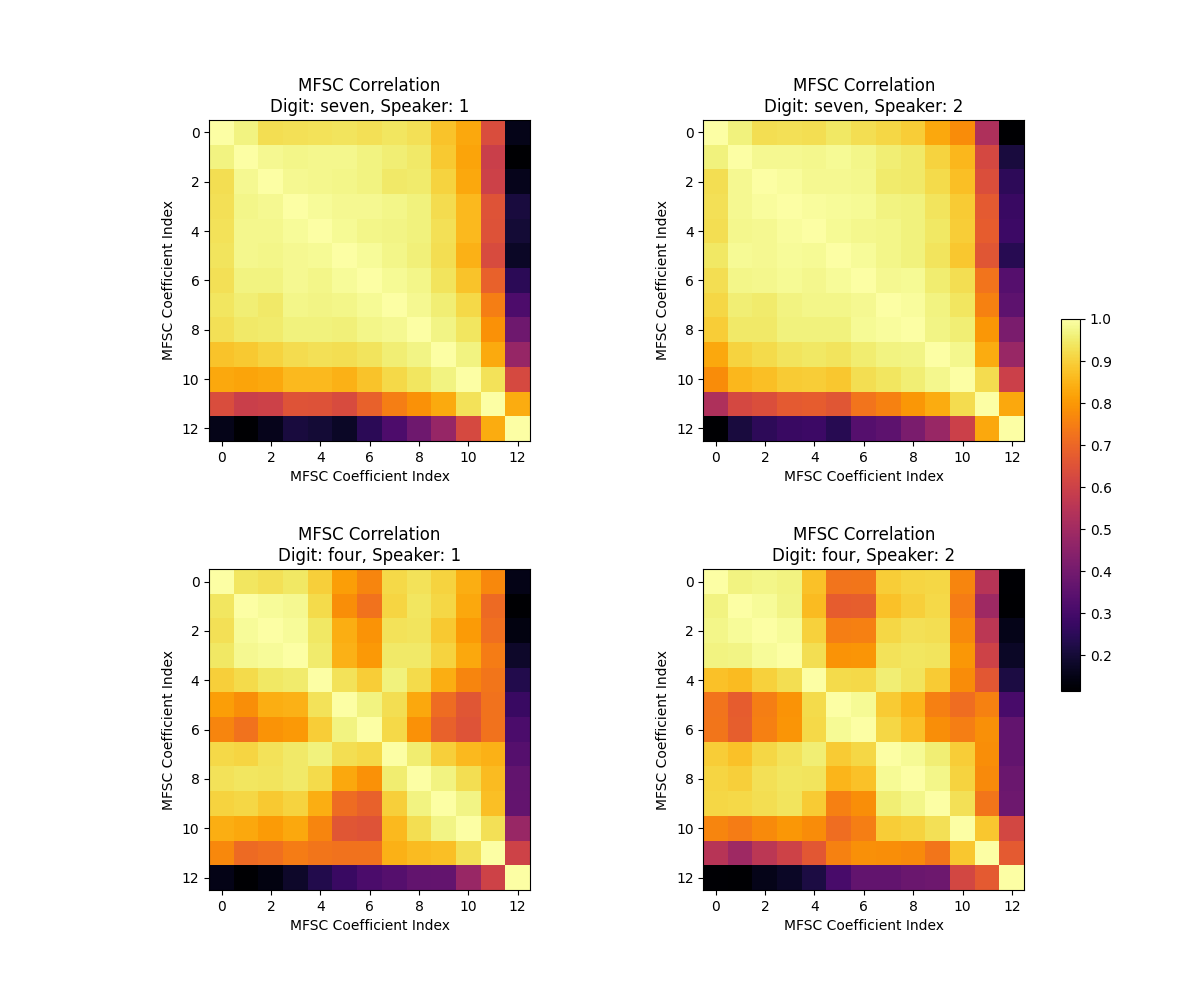
\includegraphics[width=\textwidth]{images/corr_mfsc_combined.png}
    \caption{Συσχέτιση MFSCs για τα ψηφία "seven" και "four" από δύο ομιλητές.}
    \label{fig:mfsc_correlation}
\end{figure}

\begin{figure}[h]
    \centering
    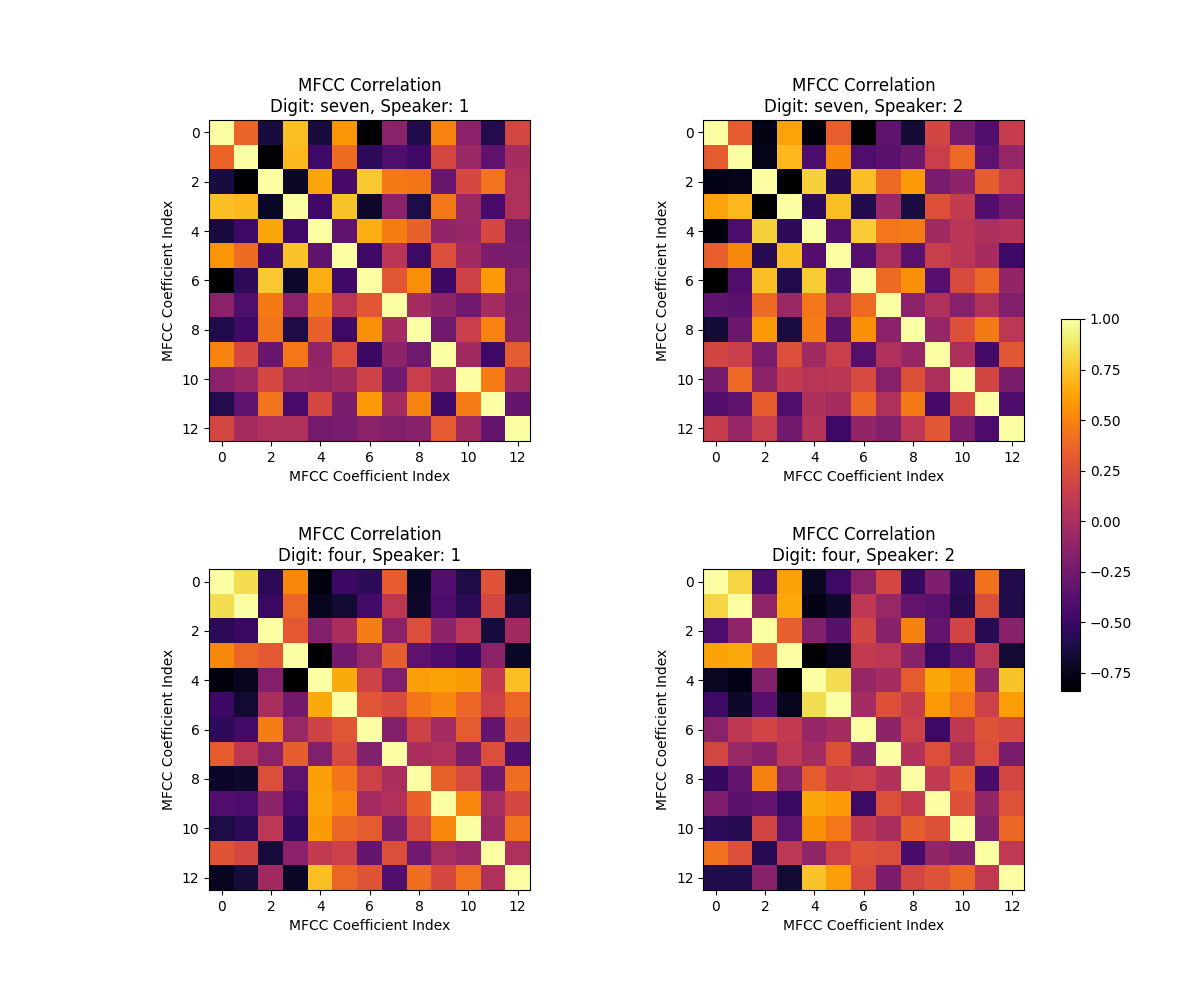
\includegraphics[width=\textwidth]{images/corr_mfcc_combined.png}
    \caption{Συσχέτιση MFCCs για τα ψηφία "seven" και "four" από δύο ομιλητές.}
    \label{fig:mfcc_correlation}
\end{figure}

\section*{Βήμα 5}

Για την προσέγγιση αναγνώρισης ψηφίων, πραγματοποιήθηκε η εξαγωγή ενός μοναδικού διανύσματος χαρακτηριστικών για κάθε εκφώνηση. Συγκεκριμένα, τα χαρακτηριστικά MFCCs, οι πρώτες διαφορές (deltas) και οι δεύτερες διαφορές (delta-deltas) συνδυάστηκαν σε ένα ενιαίο σύνολο χαρακτηριστικών. Για κάθε εκφώνηση υπολογίστηκε η μέση τιμή και η τυπική απόκλιση κάθε χαρακτηριστικού σε όλα τα παράθυρα της εκφώνησης, ώστε να προκύψει ένα διάνυσμα με συνολικά 78 διαστάσεις για κάθε εκφώνηση.

Στη συνέχεια, απεικονίστηκαν οι πρώτες δύο διαστάσεις αυτών των διανυσμάτων χαρακτηριστικών (δηλαδή η μέση τιμή και διακύμανση του πρώτου χαρακτηριστικού) σε ένα διάγραμμα διασποράς (scatter plot), όπου κάθε ψηφίο αναπαρίσταται με διαφορετικό χρώμα και σύμβολο (βλ. Εικόνα~\ref{fig:scatter_plot_feature_vectors}).

\textbf{Σχολιασμός Διαγράμματος}

Από το διάγραμμα παρατηρούμε ότι τα διαφορετικά ψηφία σχηματίζουν ξεχωριστά clusters στο χώρο των χαρακτηριστικών, κάτι που δείχνει ότι τα διανύσματα χαρακτηριστικών διαχωρίζονται επαρκώς για κάθε ψηφίο. Υπάρχουν, βέβαια, κάποιες αλληλοεπικαλύψεις μεταξύ ορισμένων ψηφίων, γεγονός που υποδηλώνει ότι ορισμένα ψηφία έχουν πιο όμοια φασματικά χαρακτηριστικά και μπορεί να χρειαστεί περαιτέρω επεξεργασία ή βελτιστοποίηση για την πλήρη διάκρισή τους.

Η διακριτότητα των clusters υποδηλώνει ότι τα MFCCs, μαζί με τις πρώτες και δεύτερες διαφορές τους,
αποτελούν αποτελεσματικά χαρακτηριστικά για την αναγνώριση ομιλίας και τον διαχωρισμό των ψηφίων. Επομένως,
η παρούσα προσέγγιση μπορεί να χρησιμοποιηθεί ως αρχική βάση για την ταξινόμηση των ψηφίων,
με πιθανή βελτίωση μέσω επιπρόσθετων τεχνικών ή ταξινομητών.

\begin{figure}[h]
    \centering
    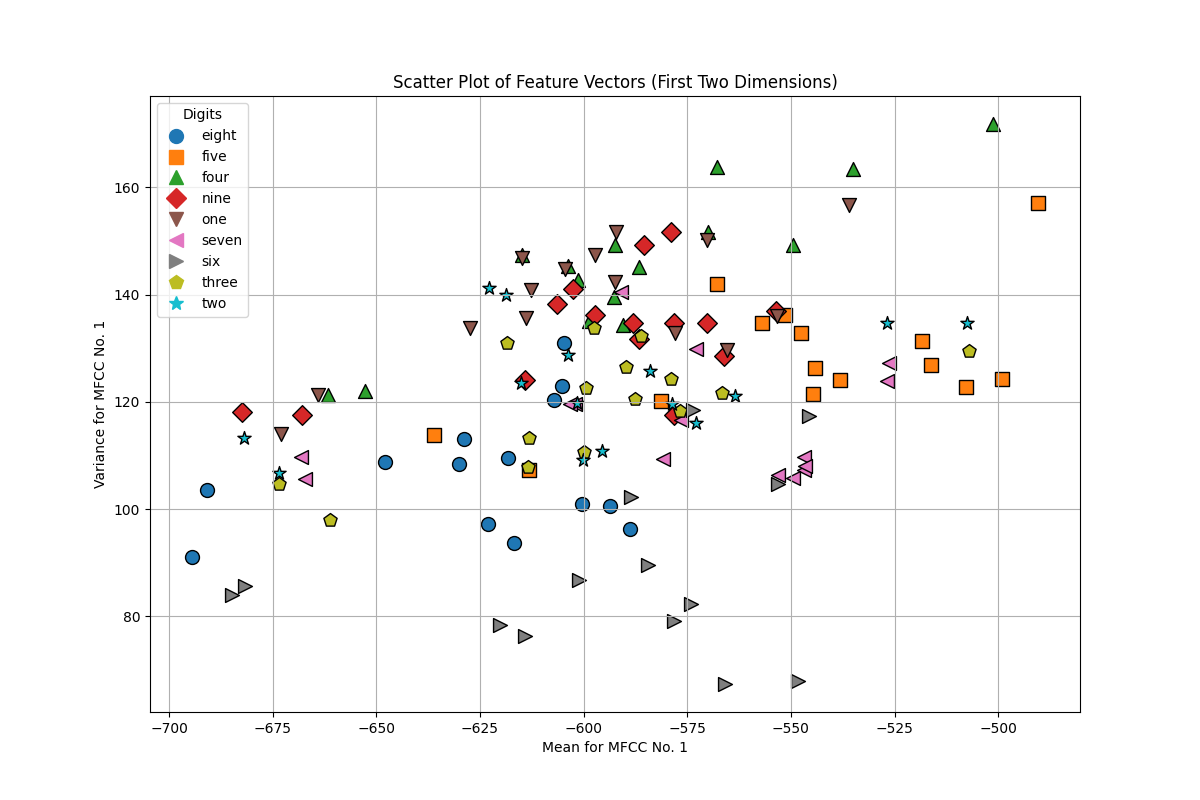
\includegraphics[width=\textwidth]{images/feature_vectors_scatterplot.png}
    \caption{Scatter Plot των διανυσμάτων χαρακτηριστικών (Πρώτες δύο διαστάσεις) για τα ψηφία "eight", "five", "four", "nine", "one", "seven", "six", "three" και "two". Κάθε ψηφίο αναπαρίσταται με διαφορετικό χρώμα και σύμβολο.}
    \label{fig:scatter_plot_feature_vectors}
\end{figure}

\section*{Βήμα 6}

Για την απεικόνιση των πολυδιάστατων διανυσμάτων χαρακτηριστικών που δημιουργήθηκαν από τα MFCCs, εφαρμόσαμε μείωση διαστάσεων μέσω Principal Component Analysis (PCA). Αρχικά, μειώσαμε τα διανύσματα σε δύο διαστάσεις και δημιουργήσαμε ένα δισδιάστατο διάγραμμα διασποράς (scatter plot), ενώ στη συνέχεια μειώσαμε σε τρεις διαστάσεις και δημιουργήσαμε ένα τρισδιάστατο scatter plot.

Σύμφωνα με τα αποτελέσματα που προέκυψαν από την ανάλυση PCA,
οι δύο πρώτες κύριες συνιστώσες διατηρούν 20.07\%
της αρχικής διασποράς των δεδομένων (11.21\% και 8.86\% για την πρώτη και δεύτερη συνιστώσα αντίστοιχα),
ενώ οι τρεις πρώτες κύριες συνιστώσες διατηρούν **28.09\% της διασποράς (11.21\%, 8.86\%, και 8.02\% για
την πρώτη, δεύτερη και τρίτη συνιστώσα αντίστοιχα). Η πληροφορία αυτή μας δείχνει ότι οι πρώτες τρεις
συνιστώσες καταφέρνουν να συγκρατήσουν σημαντικό ποσοστό της αρχικής διασποράς, αν και όχι τόσο μεγάλο ώστε να εξηγούν πλήρως τα δεδομένα.

\begin{enumerate}
    \item Στο δισδιάστατο διάγραμμα (Εικόνα~\ref{fig:pca_2d_plot}), τα σημεία που αντιπροσωπεύουν τα διαφορετικά ψηφία κατανέμονται μερικώς διακριτά, με κάποια clusters να είναι εμφανή. Ωστόσο, υπάρχει ακόμα κάποια αλληλοεπικάλυψη μεταξύ των σημείων για ορισμένα ψηφία, υποδεικνύοντας ότι η μείωση σε δύο διαστάσεις δεν είναι αρκετή για πλήρη διαχωρισμό των ψηφίων.

    \item Στο τρισδιάστατο διάγραμμα (Εικόνα~\ref{fig:pca_3d_plot}), η επιπλέον διάσταση προσθέτει λίγο περισσότερη διακριτότητα, αλλά εξακολουθούν να υπάρχουν επικαλύψεις. Η τρίτη διάσταση αυξάνει το ποσοστό της διασποράς που εξηγείται, ωστόσο η οπτική διάκριση παραμένει μερική.

\end{enumerate}

Η μείωση των διαστάσεων με PCA ήταν μερικώς επιτυχής. Αν και διατήρησε ένα σημαντικό ποσοστό της αρχικής διασποράς, οι πρώτες δύο και τρεις κύριες συνιστώσες δεν αρκούν για τον πλήρη διαχωρισμό των ψηφίων, λόγω της πολυπλοκότητας και της αλληλεξάρτησης των χαρακτηριστικών στα δεδομένα. Η προσθήκη επιπλέον συνιστωσών ενδέχεται να βοηθήσει, αλλά θα οδηγήσει σε μεγαλύτερη πολυπλοκότητα στην οπτικοποίηση. Παρ' όλα αυτά, η χρήση του PCA αποτελεί μια αποτελεσματική τεχνική για τη μείωση της διάστασης και την αρχική κατανόηση της κατανομής των χαρακτηριστικών.

\begin{figure}[h]
    \centering
    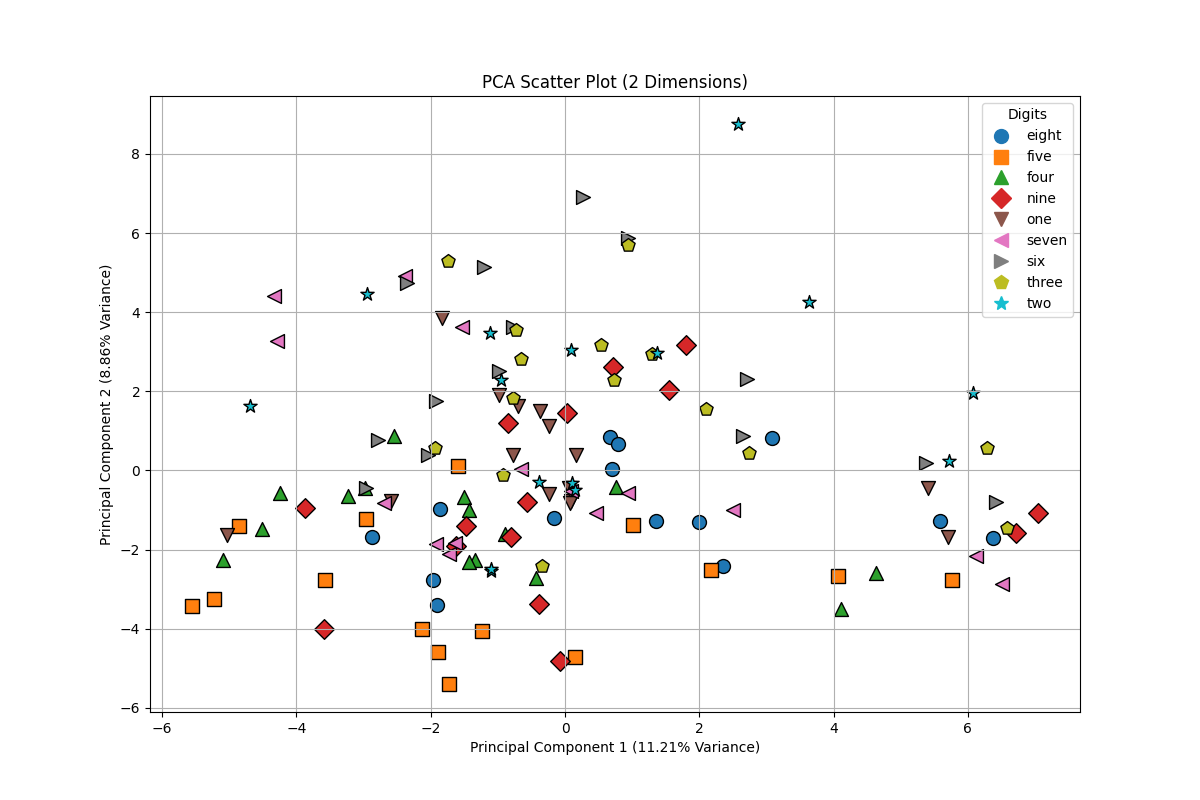
\includegraphics[width=\textwidth]{images/pca_2d_plot.png}
    \caption{PCA Scatter Plot σε δύο διαστάσεις για τα χαρακτηριστικά των ψηφίων.}
    \label{fig:pca_2d_plot}
\end{figure}

\begin{figure}[h]
    \centering
    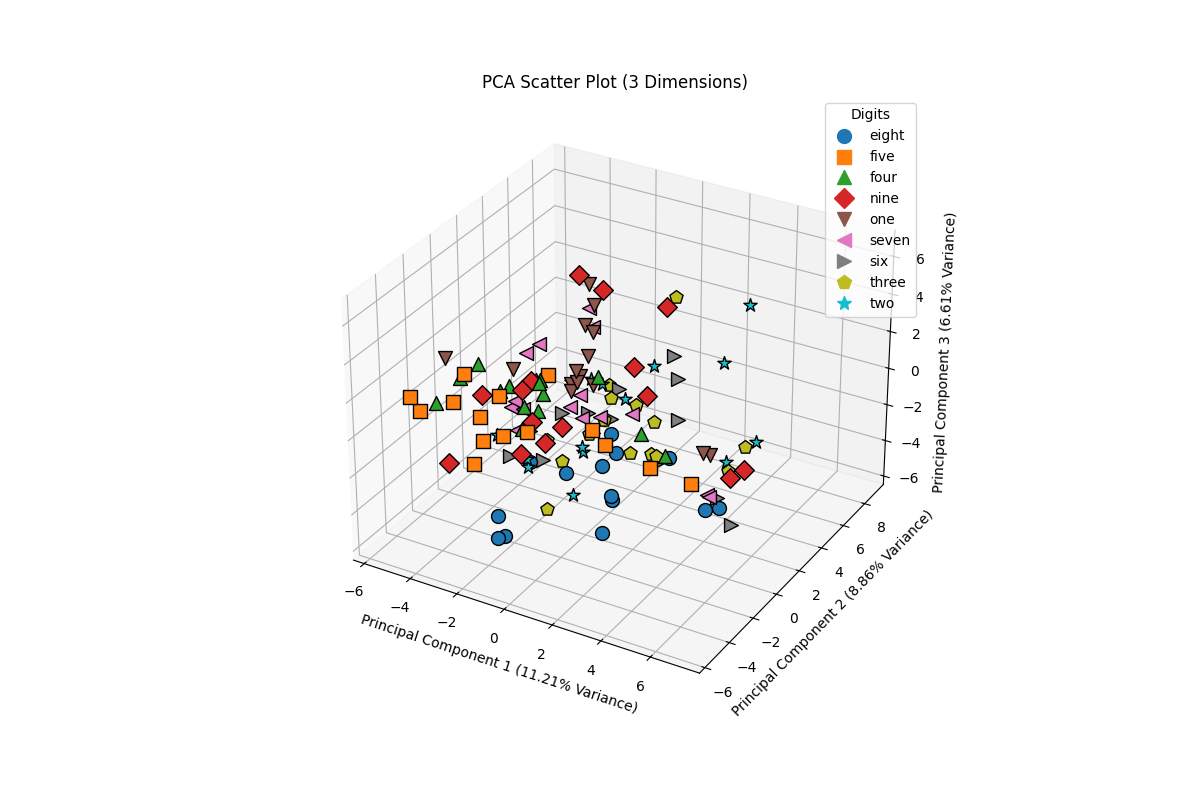
\includegraphics[width=\textwidth]{images/pca_3d_plot.png}
    \caption{PCA Scatter Plot σε τρεις διαστάσεις για τα χαρακτηριστικά των ψηφίων.}
    \label{fig:pca_3d_plot}
\end{figure}

\section*{Βήμα 7}

Για την ταξινόμηση των ηχητικών δεδομένων, ακολουθήθηκε η εξής διαδικασία:

Αρχικά, τα δεδομένα χωρίστηκαν σε σύνολα εκπαίδευσης (70\%) και ελέγχου (30\%)
χρησιμοποιώντας τη συνάρτηση \texttt{train\_test\_split} με \texttt{stratify=labels}
για να διασφαλιστεί η ισορροπημένη κατανομή των κλάσεων. Πριν την εκπαίδευση,
εφαρμόστηκε κανονικοποίηση στα δεδομένα χρησιμοποιώντας το \texttt{StandardScaler}.

Χρησιμοποιήθηκαν συνολικά 5 ταξινομητές:
\begin{enumerate}
    \item Custom Bayesian (από την πρώτη εργαστηριακή άσκηση)
    \item Gaussian Naive Bayes (από scikit-learn)
    \item SVM (με γραμμικό kernel)
    \item Random Forest (με 100 δέντρα)
    \item CatBoost
\end{enumerate}

Τα αρχικά αποτελέσματα έδειξαν παρόμοια απόδοση για όλους τους ταξινομητές:

\begin{table}[h]
    \centering
    \begin{tabular}{lcc}
        \hline
        \textbf{Ταξινομητής} & \textbf{Ακρίβεια} & \textbf{F1-Score} \\
        \hline
        Custom Bayesian      & 65.00\%           & 63.51\%           \\
        Gaussian Naive Bayes & 65.00\%           & 63.51\%           \\
        SVM                  & 65.00\%           & 62.52\%           \\
        Random Forest        & 75.00\%           & 74.88\%           \\
        CatBoost             & 67.50\%           & 65.30\%           \\
        \hline
    \end{tabular}
    \caption{Αρχικά αποτελέσματα ταξινόμησης}
\end{table}

\textbf{Bonus: Προσθήκη Επιπλέον Χαρακτηριστικών}

Για το bonus μέρος, προστέθηκαν επιπλέον χαρακτηριστικά στο διάνυσμα:

\begin{enumerate}
    \item Zero-Crossing Rate (ZCR): Αποτελεί ένα από τα βασικότερα χαρακτηριστικά στο
          πεδίο του χρόνου και υπολογίζει το ρυθμό με τον οποίο το σήμα αλλάζει πρόσημο
          \cite{kedem1986spectral}. Είναι ιδιαίτερα χρήσιμο για την αναγνώριση ομιλίας
          καθώς συσχετίζεται με το φασματικό περιεχόμενο του σήματος
          \cite{bachu2010voiced}.

    \item Πολυωνυμικά χαρακτηριστικά (Polynomial Features): Χρησιμοποιούνται για την καταγραφή της
          φασματικής παραμόρφωσης και την εκτίμηση της φασματικής περιβάλλουσας \cite{noll1967cepstrum}. Παρέχουν
          πληροφορίες για τη δομή των αρμονικών συχνοτήτων του σήματος.
\end{enumerate}

Η προσθήκη των επιπλέον χαρακτηριστικών οδήγησε σε σημαντική βελτίωση των αποτελεσμάτων:

\begin{table}[h]
    \centering
    \begin{tabular}{lccc}
        \hline
        \textbf{Ταξινομητής} & \textbf{Ακρίβεια} & \textbf{F1-Score} & \textbf{Βελτίωση Ακρίβειας} \\
        \hline
        Custom Bayesian      & 65.00\%           & 63.84\%           & 0\%                         \\
        Gaussian Naive Bayes & 65.00\%           & 63.84\%           & 0\%                         \\
        SVM                  & 72.50\%           & 72.16\%           & +7.5\%                      \\
        Random Forest        & 65.00\%           & 65.05\%           & -2.5\%                      \\
        CatBoost             & 80.00\%           & 79.99\%           & +12.5\%                     \\
        \hline
    \end{tabular}
    \caption{Αποτελέσματα μετά την προσθήκη επιπλέον χαρακτηριστικών}
\end{table}

\textbf{Συμπεράσματα}

Η σημαντική βελτίωση μπορεί να αποδοθεί στο ότι τα επιπρόσθετα χαρακτηριστικά παρείχαν
συμπληρωματική πληροφορία για τη διάκριση των ψηφίων, ιδιαίτερα το ZCR που καταγράφει
τις μεταβολές του σήματος στο πεδίο του χρόνου και τα πολυωνυμικά χαρακτηριστικά που
αποτυπώνουν επιπλέον πληροφορία στο πεδίο της συχνότητας. Ο CatBoost φαίνεται να
αξιοποίησε καλύτερα αυτή την επιπρόσθετη πληροφορία, οδηγώντας στη σημαντική βελτίωση
της απόδοσής του τόσο στην ακρίβεια όσο και στο F1-Score (79.94\%). Αξιοσημείωτη
είναι επίσης η βελτίωση του SVM, που πέτυχε F1-Score 72.16\%. Αντίθετα, οι Bayesian
ταξινομητές και ο Random Forest δεν κατάφεραν να αξιοποιήσουν αποτελεσματικά τα
επιπλέον χαρακτηριστικά.

\section*{Βήμα 8}

\section*{Αναγνώριση Ψηφίων με GMM-HMM}

\subsection*{Βήμα 9: Διαχωρισμός Δεδομένων}

Αρχικά, τα δεδομένα εκπαίδευσης διαχωρίστηκαν σε training και validation set με αναλογία 80\%-20\% χρησιμοποιώντας τη συνάρτηση \texttt{train\_test\_split} της βιβλιοθήκης scikit-learn. Η παράμετρος \texttt{stratify=labels} εξασφάλισε την ισορροπημένη κατανομή των ψηφίων στα δύο σύνολα:

\begin{verbatim}
X_train, X_val, y_train, y_val, spk_train, spk_val = train_test_split(
   X, y, spk, test_size=0.2, random_state=42, stratify=y)
\end{verbatim}

\subsection*{Βήμα 10: Υλοποίηση GMM-HMM}

\subsubsection*{Αρχικοποίηση Μοντέλου}
Υλοποιήθηκε ένα GMM-HMM μοντέλο για κάθε ψηφίο, με δυνατότητα παραμετροποίησης των εξής χαρακτηριστικών:
\begin{itemize}
    \item \texttt{n\_states}: Αριθμός καταστάσεων HMM (1-4)
    \item \texttt{n\_mixtures}: Αριθμός Gaussian κατανομών στο μείγμα (1-5)
    \item Δυνατότητα επιλογής μεταξύ απλής Gaussian και GMM κατανομής
\end{itemize}

\subsubsection*{Δομή Left-Right HMM}
Ο πίνακας μεταβάσεων $A = \{a_{ij}\}$ αρχικοποιήθηκε ως left-right με τους εξής περιορισμούς:
\begin{itemize}
    \item Για μία κατάσταση:
          \begin{itemize}
              \item $a_{00} = 1$ (πλήρης αυτομετάβαση)
          \end{itemize}
    \item Για πολλαπλές καταστάσεις:
          \begin{itemize}
              \item $a_{ij} = 0$ για $j < i$ (απαγόρευση μεταβάσεων προς τα πίσω)
              \item $a_{ij} = 0$ για $j > i + 1$ (επιτρέπονται μόνο μεταβάσεις σε διαδοχικές καταστάσεις)
              \item $a_{ii} = 0.5$ για $i < n-1$ (πιθανότητα παραμονής στην ίδια κατάσταση)
              \item $a_{i,i+1} = 0.5$ για $i < n-1$ (πιθανότητα μετάβασης στην επόμενη κατάσταση)
              \item $a_{n-1,n-1} = 1$ (η τελευταία κατάσταση είναι απορροφητική)
          \end{itemize}
    \item Αρχικές πιθανότητες: $\pi_i = \begin{cases} 1 & \text{για } i = 1 \\ 0 & \text{για } i \neq 1 \end{cases}$
    \item Τελικές πιθανότητες: $f_i = \begin{cases} 1 & \text{για κατάσταση } i = n \text{ ή } n=1 \\ 0 & \text{αλλιώς} \end{cases}$
\end{itemize}

\subsection*{Εκπαίδευση με τον Αλγόριθμο EM (Baum-Welch)}
Η εκπαίδευση των μοντέλων πραγματοποιήθηκε με τον αλγόριθμο Baum-Welch μέσω της βιβλιοθήκης Pomegranate:
\begin{verbatim}
model = DenseHMM(
   distributions=emission_model,
   edges=A,
   starts=start_probs,
   ends=end_probs,
   verbose=True,
   max_iter=100,
   tol=1e-3
).fit(data)
\end{verbatim}

Για κάθε κατάσταση, οι κατανομές εκπομπής προσαρμόζονται στα δεδομένα με δύο τρόπους:
\begin{itemize}
    \item \textbf{GMM}: Μείγμα Gaussian κατανομών με n\_mixtures συνιστώσες
    \item \textbf{Απλή Gaussian}: Μία Gaussian κατανομή ανά κατάσταση
\end{itemize}

Ο αλγόριθμος εκτελείται μέχρι:
\begin{itemize}
    \item Να φτάσει τις 100 επαναλήψεις (\texttt{max\_iter=100})
    \item Ή η μεταβολή της πιθανοφάνειας να είναι μικρότερη από $10^{-3}$ (\texttt{tol=1e-3})
\end{itemize}

\subsection*{Αξιολόγηση Μοντέλου}
Για την αξιολόγηση του μοντέλου:
\begin{itemize}
    \item Υπολογίζεται ο λογάριθμος της πιθανοφάνειας (\texttt{log\_probability}) για κάθε ακολουθία και κάθε μοντέλο
    \item Επιλέγεται το μοντέλο (ψηφίο) με τη μέγιστη πιθανοφάνεια ως πρόβλεψη
    \item Υπολογίζεται το σκορ ακρίβειας στο validation και test set
    \item Δημιουργούνται κανονικοποιημένα Confusion Matrix για την οπτικοποίηση των αποτελεσμάτων
\end{itemize}

% Insert image
\begin{figure}[h]
    \centering
    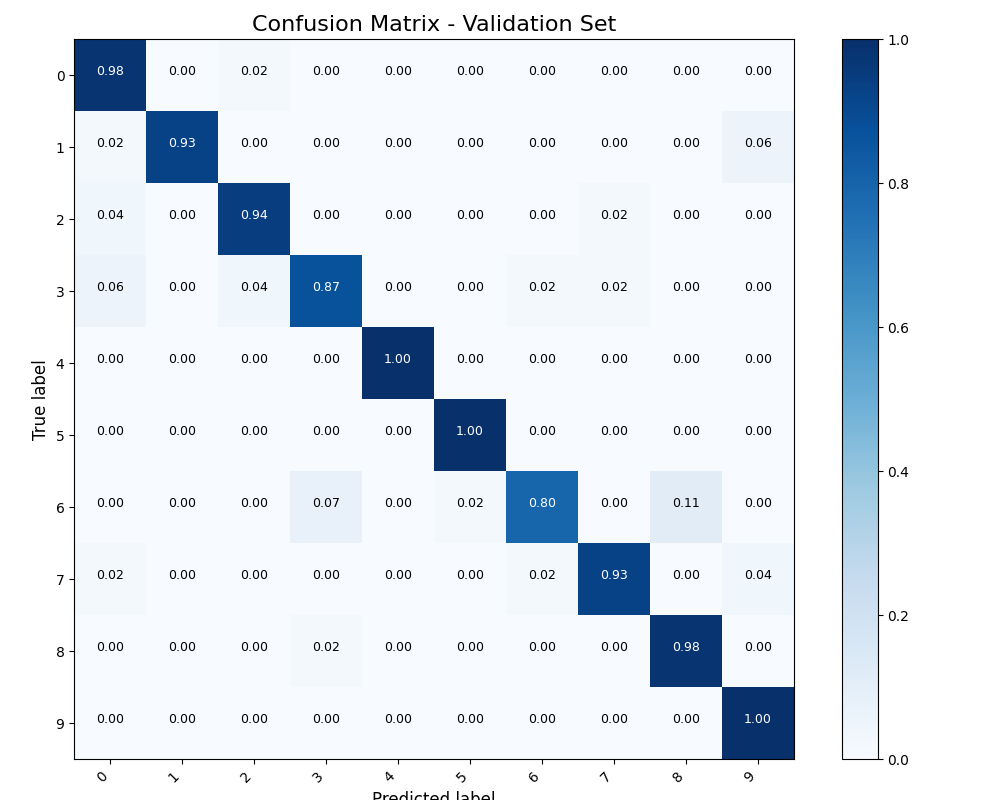
\includegraphics[width=0.8\textwidth]{hmm_val_cm.png}
    \caption{Κανονικοποιημένο Validation Confusion Matrix για το μοντέλο GMM-HMM}
    \label{fig:hmm_confusion_matrix}
\end{figure}

\begin{figure}{h}
    \centering
    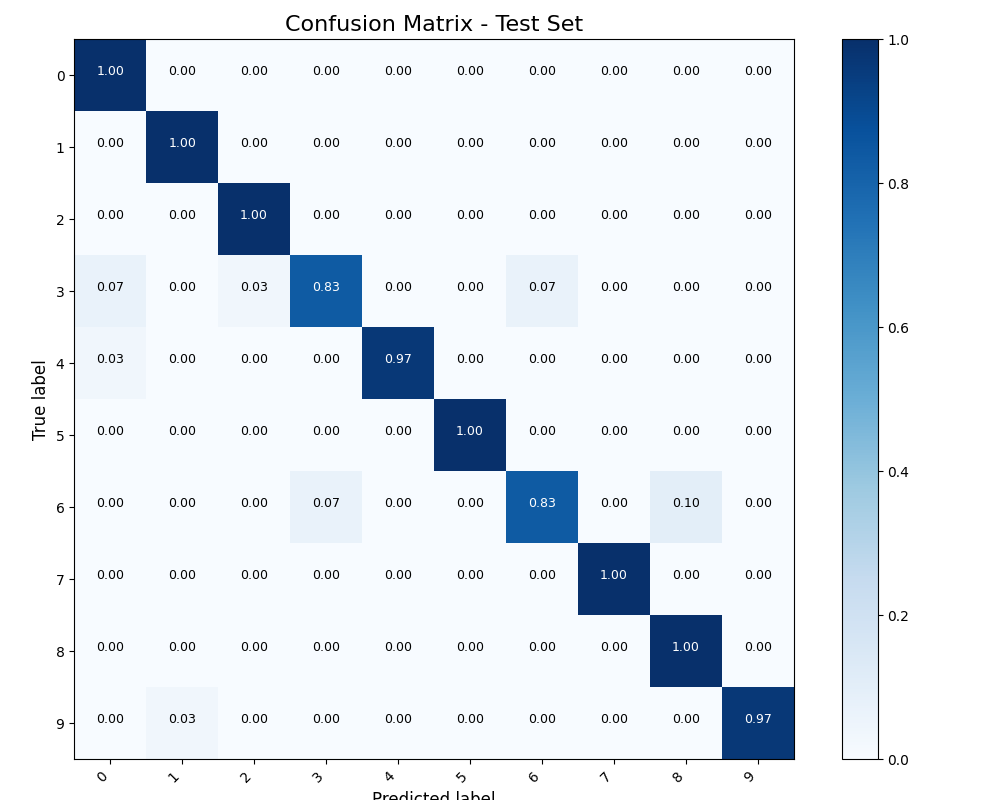
\includegraphics[width=0.8\textwidth]{hmm_test_cm.png}
    \caption{Κανονικοποιημένο Test Confusion Matrix για το μοντέλο GMM-HMM}
    \label{fig:hmm_confusion_matrix}
\end{figure}



\subsection*{Εκπαίδευση Μοντέλων (Βήμα 11)}
Για την αναγνώριση ψηφίων, εκπαιδεύτηκαν 10 ξεχωριστά GMM-HMM μοντέλα (ένα για κάθε ψηφίο) με τον αλγόριθμο Expectation-Maximization. Διερευνήθηκε ένα εύρος παραμέτρων με:
\begin{itemize}
    \item Αριθμό καταστάσεων HMM: 1 έως 4
    \item Αριθμό Γκαουσιανών κατανομών: 1 έως 5
\end{itemize}

Η εκπαίδευση πραγματοποιήθηκε με τα εξής χαρακτηριστικά:
\begin{itemize}
    \item Μέγιστος αριθμός επαναλήψεων: 100
    \item Κριτήριο σύγκλισης: μεταβολή του λογαρίθμου πιθανοφάνειας < $10^{-3}$
    \item Χρήση όλων των διαθέσιμων δεδομένων για κάθε ψηφίο
\end{itemize}

\subsection*{Διαδικασία Αναγνώρισης και Αξιολόγησης (Βήμα 12)}
Μετά την εκπαίδευση, η αξιολόγηση πραγματοποιήθηκε σε δύο στάδια:
\begin{enumerate}
    \item Αρχική αξιολόγηση στο validation set για την εύρεση βέλτιστων παραμέτρων
    \item Τελική αξιολόγηση στο test set με τις βέλτιστες παραμέτρους
\end{enumerate}

Η διαδικασία αναγνώρισης για κάθε εκφώνηση περιελάμβανε:
\begin{itemize}
    \item Υπολογισμό του λογαρίθμου πιθανοφάνειας για κάθε μοντέλο
    \item Επιλογή του μοντέλου με τη μέγιστη πιθανοφάνεια ως τελική πρόβλεψη
\end{itemize}

\begin{figure}[h]
    \centering
    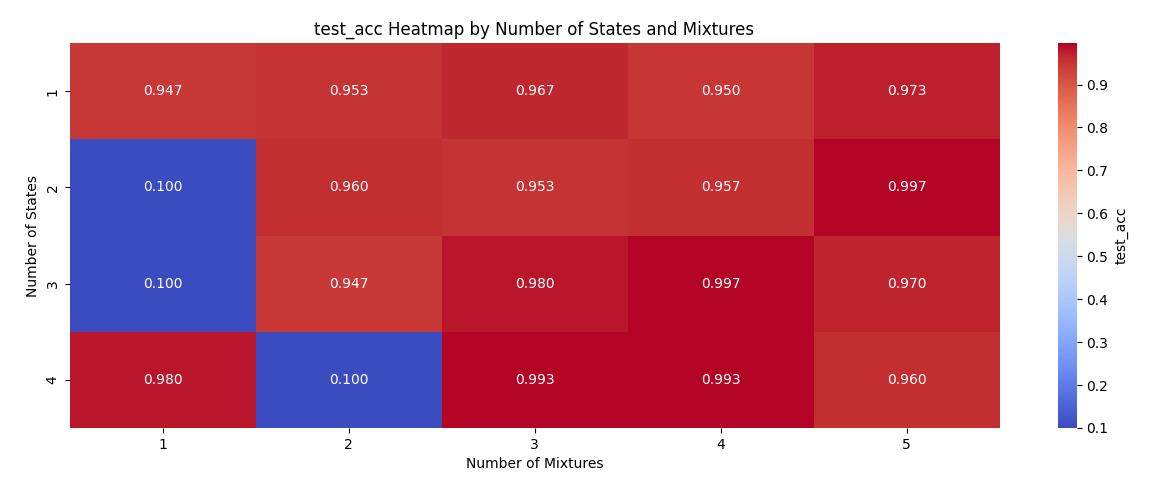
\includegraphics[width=0.8\textwidth]{hmm_test_acc_heatmap.png}
    \caption{Χάρτης θερμότητας ακρίβειας στο test set ως προς τον αριθμό καταστάσεων και μειγμάτων. 
    Οι τιμές αντιπροσωπεύουν το ποσοστό ακρίβειας (accuracy) για κάθε συνδυασμό παραμέτρων. 
    Σκοτεινότερο κόκκινο υποδεικνύει υψηλότερη ακρίβεια, ενώ το μπλε χαμηλότερη.}
    \label{fig:test_acc_heatmap}
\end{figure}

\subsection*{Ανάλυση Αποτελεσμάτων (Βήμα 13)}
Όπως φαίνεται στο Σχήμα \ref{fig:test_acc_heatmap}, τα αποτελέσματα της αξιολόγησης στο test set έδειξαν:

\subsubsection*{Επίδραση Παραμέτρων}
\begin{itemize}
    \item \textbf{Βέλτιστη επίδοση}: 99.7\% ακρίβεια με 2 καταστάσεις και 5 μείγματα Γκαουσιανών
    \item \textbf{Αριθμός καταστάσεων}:
          \begin{itemize}
              \item 2-3 καταστάσεις παρουσίασαν σταθερά υψηλή απόδοση
              \item 4 καταστάσεις έδειξαν μεγαλύτερη διακύμανση στην απόδοση
          \end{itemize}
    \item \textbf{Αριθμός μειγμάτων}:
          \begin{itemize}
              \item Αύξηση του αριθμού μειγμάτων γενικά βελτίωσε την απόδοση
              \item 3-5 μείγματα έδωσαν σταθερά καλά αποτελέσματα
          \end{itemize}
\end{itemize}

\subsubsection*{Σημαντικά Ευρήματα}
\begin{itemize}
    \item Υψηλή απόδοση (>95\%) για τις περισσότερες σταθερές διαμορφώσεις
    \item Ορισμένοι συνδυασμοί παραμέτρων (π.χ., 2-3 καταστάσεις με 1 μείγμα) έδειξαν πολύ χαμηλή απόδοση (10\%)
    \item Σταθερή υψηλή απόδοση στην περιοχή 3+ μειγμάτων για όλες τις καταστάσεις
\end{itemize}

Η διαδικασία αξιολόγησης σε δύο στάδια (validation και test) αποδείχθηκε κρίσιμη για:
\begin{itemize}
    \item Αποφυγή υπερπροσαρμογής (overfitting)
    \item Εύρεση βέλτιστων παραμέτρων χωρίς μεροληψία
    \item Αξιόπιστη εκτίμηση της πραγματικής απόδοσης του μοντέλου
\end{itemize}

Τα αποτελέσματα επιβεβαιώνουν την αποτελεσματικότητα της προσέγγισης GMM-HMM για την αναγνώριση μεμονωμένων ψηφίων, 
με το μοντέλο να επιτυγχάνει εξαιρετική ακρίβεια στις βέλτιστες διαμορφώσεις του.

\bibliographystyle{plainnat}
\bibliography{references}

\end{document}